\chapter{Defining some concepts and redifining the variables} \label{section:bass}
Before we start this section, we need to look at some vocabulary to make sure we understand what we are discussing. Here we will define the terms "parts" and "registers". In an n-voice composition, there are n registers and n parts. The parts correspond to what a given individual sings, in other words, each part corresponds to a staff. This is the same term that Fux uses in his work. The \textit{cantus firmus}, like each of the counterpoints, are parts.
As for the registers, these are each of the melodic lines, starting from the lowest to the highest. The lowest register always consists of the lowest notes of all the parts. This term has been chosen because it is close to its original meaning, which is that in music the term "register" refers to the entire pitch range covered by a musical composition, encompassing the low, middle and high frequencies of the audible spectrum. 
We will use these terms where the distinction between the concepts is important; where it is not, we will also use the generic term 'voice'.
Since a picture is worth a thousand words, Figure \ref{fig:lowest} illustrates the difference between parts (the blue lines) and registers (the red and orange lines). The lowest register is shown in its own colour (red) because it will be particularly important later on.

\begin{figure}[ht]
  \centering
  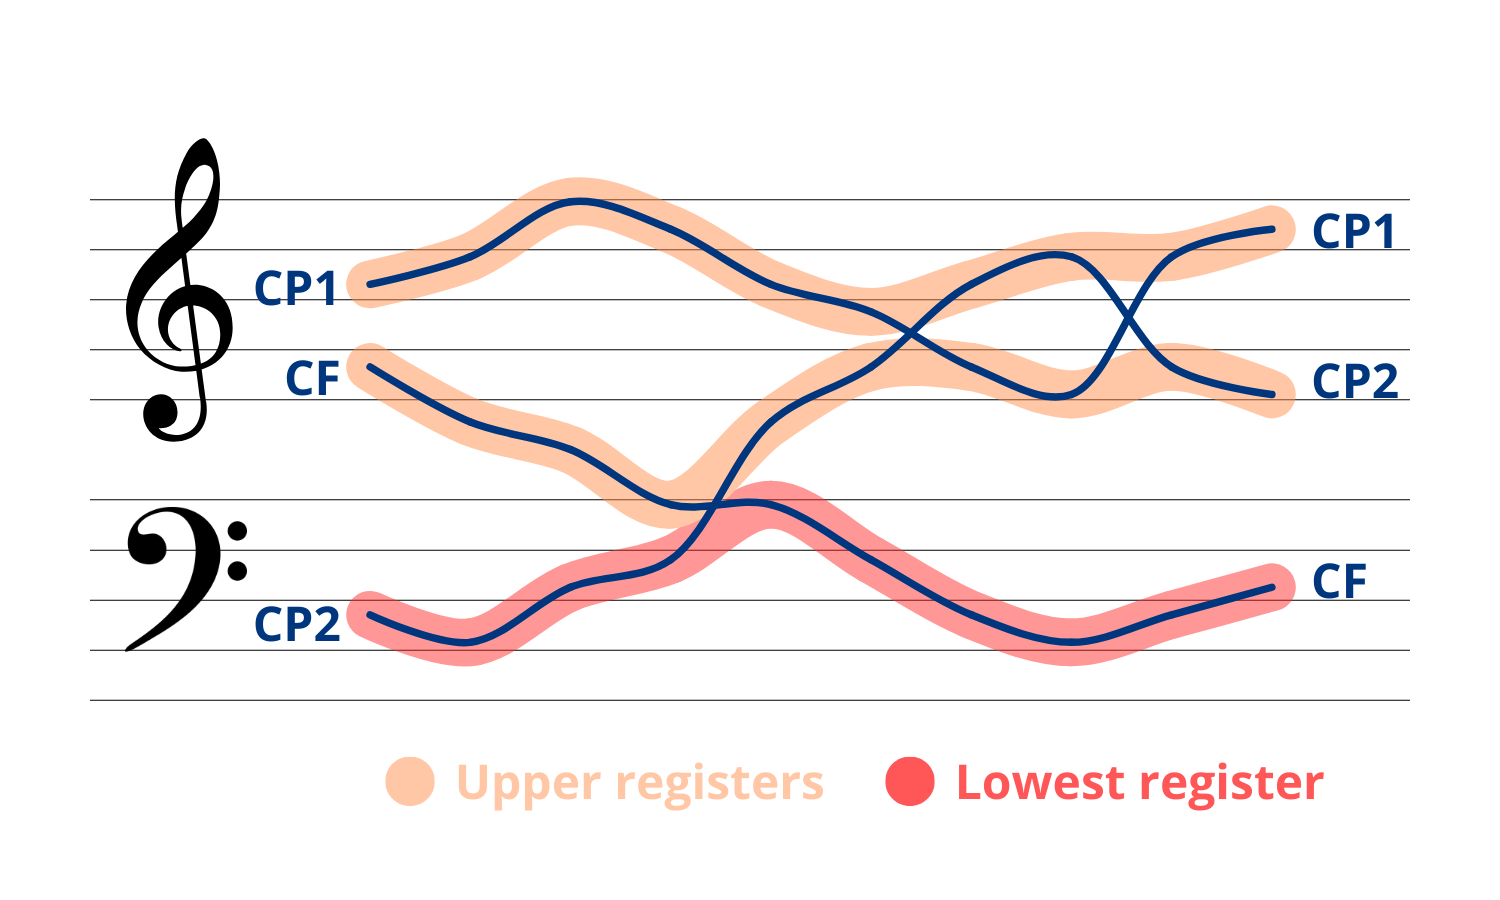
\includegraphics[width=1\textwidth]{Images/lowest.png}
  \caption{Parts and registers in a three voice composition}
  \label{fig:lowest}
\end{figure}

Here is also the mathematical representation of the lowest register (written $N^{\lambda}$, see section \ref{section:changes induced} for the notations):
\begin{equation}
    \forall j \in [0, m-1) : N^{\lambda}[0,j] = min(N^{cp_1}[0,j], N^{cp_1}[0,j], N^{cp_1}[0,j])
\end{equation}

Of the first upper register, or medium register (written $N^{u_1}$):
\begin{equation}
    \forall j \in [0, m-1) : N^{u_1}[0,j] = med(N^{cp_1}[0,j], N^{cp_1}[0,j], N^{cp_1}[0,j])
\end{equation}

And of the second upper register, or uppest register (written $N^{u_2}$):
\begin{equation}
    \forall j \in [0, m-1) : N^{u_2}[0,j] = max(N^{cp_1}[0,j], N^{cp_1}[0,j], N^{cp_1}[0,j])
\end{equation}

One of the major differences between the implementation of two-voice counterpoint (i.e., one \textit{cantus firmus} and one counterpoint) and the generalisation to three voices (i.e., one \textit{cantus firmus} and two counterpoints) is that the rules no longer necessarily apply between the counterpoints and the \textit{cantus firmus}. If we go back to the rules for two voices, we see that each of them applied between the single counterpoint and the \textit{cantus firmus}. For example, when it was stated that each interval must be consonant, this referred to the interval between the counterpoint and the \textit{cantus firmus}.
On the other hand, in his second part (where he describes the rules for composing in three voices), Fux explains that the rules are not necessarily to be observed between each of the counterpoints and the \textit{cantus firmus}, but rather between each of the voices and the lowest voice. Again, if we take the example of the need for consonance between the voices, consonance will be required in the intervals between the notes of a voice and those of the bass (whether or not the latter is the \textit{cantus firmus}).
Fux also points out that the lowest voice can change, and that at any given moment the lowest voice should be considered. In other words, Fux says that the rules apply between the parts and the lowest register.
This may seem trivial, but it's a huge paradigm shift, because the relationships are no longer considered in the same way! The \textit{cantus firmus} loses some of its pride of place and cedes much of it to the lowest register.
In fact, it's only a change in appearance. From the beginning, when there were only two voices, the rules applied between each voice and the lowest register. Now, when there is only one counterpoint and one \textit{cantus firmus}, the lower register will always be equal to one and the other will be the bass, and when the rules are applied between the single counterpoint and the \textit{cantus firmus}, the rules are necessarily applied 'equally' between the upper voice and the lower voice. Two-part counterpoint was therefore a special case of a more general rule, which it nevertheless follows!

It is, of course, possible for the \textit{cantus firmus} to be the lower voice, in which case nothing changes in the way the problem is perceived. It's when it ends up higher than one of the counterpoints that this consideration becomes important.

A very important detail about this and maybe the biggest change brought about by this paradigm shift is that the \textit{cantus firmus} now becomes a counterpoint like any other, with the difference that its notes are already fixed. This means that we are going to treat the \textit{cantus firmus} as a first species counterpoint (since it is always constituted by only whole notes), and that we will need to calculate its intervals, movements and costs, as we have already been doing it with 'normal' counterpoints.

\section{Changes induced in the variables} \label{section:changes induced}

Many changes have been induced as a result of the three part generalisation. In two part composition, it was obvious that the harmonic intervals array was describing the intervals between the \textit{cantus firmus} and the only counterpoint, it was obvious that the motions were those of the only counterpoint, and so it goes for all the variables. When writing a three part composition, we are dealing with many possibilities when speaking about "intervals" or motions. Intervals between which voices? Motions of which counterpoint? To tackle this, each variable is now related to a voice.

When written in the exponent of a variable, $cf$ means that the variable is related to the \textit{cantus firmus}. $cp_1$ means that the variable is about the first counterpoint and $cp_2$ means that the variable is about the second one.

When a variable is about the lowest register, its exponent is \textit{$\lambda$} (this notation was chosen because it is much easier to read than a simple \textit{l}). The top voices are denoted \textit{u$_1$} and \textit{u$_2$} (for "\textit{u}pper").

The notation H$^{cp_1}$, for example, corresponds to the variable representing the harmonic intervals of the first counterpoint, whereas H$^{cf}$ are the harmonic intervals of the bass (see section \ref{subsection:modified_variables} what this actually means).

This change applies to all variables (i.e. N (formerly cp), H, M, P, IsCfB and IsCons) and to all costs (section 2.2.2 of T. Wafflard's thesis) with the exception of $\mathcal{C}$ (the cost factors) and $\tau$ (the total cost).

\subsection{Added variables}
\vspace{.5cm} \noindent \textbf{$\Lambda$} \hspace{.cm} \texttt{is-bass} \label{is-bass}

This boolean array of size $m$ reifies if the considered part is the lowest one. Its notation was chosen as it is the uppercase of $\lambda$ (the lowest register). It only takes into consideration the first note of every measure. The reason for this is that when all the rules were given according to the \textit{cantus firmus}, they were always based on the first beat of each measure (which is logical, as the \textit{cantus firmus} has no notes on the other beats. Given that the rules should work exactly the same way, they are only considering the first beat of the lowest record.
It is also worth to be noted that only one of the parts can be the lowest record at the time. This does not mean that two parts cannot equal the lowest record at the same time, they can. It means that only one of those two is going to be considered to \textit{be} the lowest record (and the other one will be the middle record). This is needed in order for motions to work well (both the motions costs and the constraint not to get to a direct consonance by direct motion).

Here is the mathematical definition of this array:
\begin{equation}
\begin{aligned}
&\forall j \in [0, m-1) \colon  \\
\Lambda^{cf}[j] &:= (N^{cf}[0,j] = N^\lambda[0,j])\\
\Lambda^{cp_1}[j] &:= ((N^{cp_1}[0,j] = N^\lambda[0,j]) \land \neg \Lambda^{cf}[j])\\
\Lambda^{cp_2}[j] &:= (\neg \Lambda^{cf} \land \neg \Lambda^{cp_1})
\end{aligned}
\end{equation}

In practice, there is only a \texttt{is-not-bass} array in the code (which is then equal to $\neg \Lambda$), as it is almost always more useful to know if a part is \textit{not} the lowest record than knowing if it is the lowest one. 


\subsection{Modified variables} \label{subsection:modified_variables}
Given that the majority of the rules now apply between parts and the lowest register, the meaning of the variables has been modified to adapt to this reality. 

\vspace{.5cm} \noindent \textbf{N} \hspace{.2cm} \texttt{notes} 

We changed the name of former \texttt{cp} array and renamed it to \texttt{N} (for notes), for the sake of clarity. As we have now three of those arrays (one for the first counterpoint, one for the second counterpoint, and even one for the \textit{cantus firmus}), it needed a less ambiguous name than the one it had before.


\vspace{.5cm} \noindent \textbf{H}$_{(abs)}^{v_1-v_2}$ \hspace{.2cm} \texttt{h-intervals}\hspace{.2cm} \texttt{h-intervals-abs}\hspace{.2cm} \texttt{h-intervals-to-cf}\hspace{.2cm} \texttt{h-intervals-cp1-to-cp2}

The way in which this variable works remains much the same, i.e. it represents the interval between one voice and another. This definition has been extended to include intervals other than that between the counterpoint and the \textit{cantus firmus}. Thus, H$^{v1-v2}$ represents the intervals between the $i$th beat of voice $v_1$ and the \textit{first} beat of voice $v_2$. By default, H$^{v_1}$ represents the intervals between the voice $v_1$ and the lowest register, so $H^{v_1} := H^{v_1-\lambda}$.

Here is a generalisation of the previous rule, matching to the current definition of the harmonic intervals array:
\begin{equation}
\begin{aligned}
    &\forall i \in \mathcal{B}, \quad \forall j \in [0, m) \quad \forall v_1, v_2 \in \{cf, cp_1, cp_2\}, v_1 \neq v_2:\\
    &H_{abs}^{v_1-v_2}[i, j] = \left|N^{v_1}[i, j] - N^{v_2}[0,j]\right|\\
    &H^{v_1-v_2}[i, j] = H_{abs}[i, j]\ \text{mod}\ 12\\
    &\text{where } H_{abs}[i, j] \in [0, 127], H[i, j] \in [0, 11]
\end{aligned}
\end{equation}


\vspace{.5cm}
\noindent \textbf{P} \hspace*{.2cm} \texttt{motions}

Motions are now calculated according to the movements of the lowest register. The problem here is that if a part is also the lowest register, we end up calculating the motion between a part and itself. This inevitably leads to direct motions being calculated, because a part is always moving in the same direction as itself. To solve this problem, the motions of a part are now equal to -1 when the part is also the lowest record (denoted $\Lambda$, see section \ref{is-bass}). 
\begin{equation}
\begin{aligned}
&\forall v \in \{cf, cp_1, cp_2\}, \quad \forall x \in \{1, 2\}, \quad \forall i \in B, \quad \forall j \in [0, m - 1),\quad x := b - i\\
    P^{v}[i,j]& = \,  
    \begin{cases}
        -1 & \text{if } \Lambda^{v} \\
        0 & \text{if } \neg \Lambda^{v} \land ((M_{brut}^{x, v}[i, j] > 0 > M^{\lambda}_{brut}[j]) \vee\, (M_{brut}^{x, v}[i, j] < 0 < M^{\lambda}_{brut}[j])) \\
        1 & \text{if } \neg \Lambda^{v} \land (M_{brut}^{x, v}[i, j] = 0  \oplus M^{\lambda}_{brut}[j]=0) \\
        2 & \text{if } \neg \Lambda^{v} \land ((M_{brut}^{x, v}[i, j] > 0 \land M^{\lambda}_{brut}[j] > 0) \vee\, (M_{brut}^{x, v}[i, j] < 0 \land M^{\lambda}_{brut}[j] <0))
    \end{cases}
\end{aligned}
\end{equation}
